Ce tri consiste à diviser le problème initial en sous problèmes et les
résoudre un par un.

Ce tri se décompose en trois étapes :
\begin{enumerate}
  \item Diviser
  \item Regner
  \item Combiner
\end{enumerate}

\begin{figure}[h]
\centering
\fbox{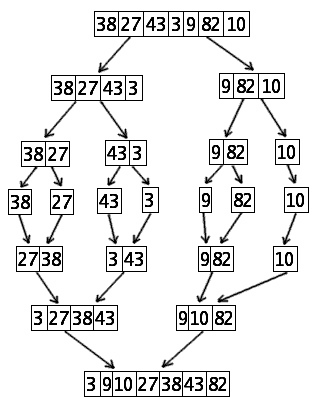
\includegraphics[scale=0.67]{images/trifusion.png}}
\caption{Fonctionnement du tri fusion}
\end{figure}

\begin{lstlisting}
TRI_FUSION(debut, fin, A) FAIRE
  SI (debut<fin)
  ALORS
    pivot <- (debut+fin)/2
    TRI_FUSION(debut, pivot, A)
    TRI_FUSION(pivot+1, fin, A)
    FUSION(debut, pivot, fin, A)
  FIN SI
FIN
\end{lstlisting}

\subsection{Calcul du coût}
Un algorithme récursif entraîne une équation récursive. 

Pour un tableau $A$ donné, il possède $n$ éléments.

Le coût global d'execution $\theta$ est 
$T(n) = aT(\frac{n}{b}) + D(n) + C(n)$ où $\frac{n}{b}$ représente la taille
des sous-problèmes et $a$ le nombre de sous problèmes.

$D(n)$ correspond à la partie \textit{diviser}. Il possède un coût constant
$O(1)$.

$C(n)$ correspond à la partie \textit{combiner}. Il possède un coût linéaire
$O(n)$.

Enfin, la partie \textit{régner} est représentée par $T(n)$. On prendra
$a=2, b=2$.

\begin{align*}
T(n) &= 2T(\frac{n}{2}) + O(1) + O(n)\\
     &= 2T(\frac{n}{2}) + O(n)\\
\end{align*}
\begin{align*}
T(\frac{n}{2}) &= 2T(\frac{n}{4}) + O(\frac{n}{2})\\
T(\frac{n}{4}) &= 2T(\frac{n}{8}) + O(\frac{n}{4})\\
T(\frac{n}{8}) &= 2T(\frac{n}{16}) + O(\frac{n}{8})\\
T(2) &= 2T(1) + O(1)\\
\end{align*}
\begin{align*}
T(n) &= 2^2T(\frac{n}{4}) + 2O(\frac{n}{2}) + O(n)\\
     &= 2^2(2T(\frac{n}{8}) + O(\frac{n}{4})) + 2O(\frac{n}{2}) + O(n)\\
     &= 2^3T(\frac{n}{2^3}) + 2^2O(\frac{n}{2^2}) + 2O(\frac{n}{2}) + O(n)\\
\end{align*}
\begin{align*}
T(n) &= \displaystyle{\sum^{log_2n}_{i=1}}2^iT(\frac{n}{2^i}) +
2^{i-1}O(\frac{n}{2^{i-1}})\\
     &= nT(1) + log_inO(n)\\
     &= nO(1) + O(nlog_2n) = O(n) + O(nlogn)\\
     &= O(nlogn)\\
\end{align*}

$$T(n) = \left\{\begin{array}{ll}
aT(\frac{n}{b}) + \underbrace{D(n) + C(n)}_{f(n)} & \mbox{ si $n > n_0$}\\
O(1) & \mbox{ si $n \le n_0$}
\end{array}\right.$$

Nous avons donc $T(n) = \underbrace{O(n^{log_ba})}_{\text{Complexité d'une
feuille de l'arbre}} + \underbrace{\displaystyle{\sum^{b}_{i=0}}a^if(
\frac{n}{b^i})}_{\text{Complexité d'un nœud interne de l'arbre}}$

\subsubsection{Théorème général}

$$T(n) = \left\{\begin{array}{ll}
aT(\frac{n}{b}) + \underbrace{D(n) + C(n)}_{f(n)} & \mbox{ si $n > n_0$}\\
O(1) & \mbox{ si $n \le n_0$}
\end{array}\right.$$

Il existe trois cas :
\begin{description}
  \item[$f(n) = O(n^{log_ba - \Sigma})$] alors $T(n) = O(n^{log_ba})$
  \item[$f(n) = O(n^{log_ba})$] alors $T(n) = O(n^{log_ba}log n)$
  \item[$f(n) = \Omega(n^{log_ba})$] alors $T(n) = O(f(n))$
\end{description}
